\documentclass[border=2mm]{standalone}
\usepackage[utf8]{inputenc}
\usepackage{tikz}
\usepackage{newtxtext,newtxmath}
\begin{document}
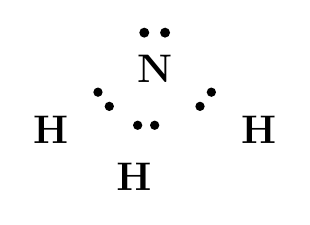
\begin{tikzpicture}[font=\bfseries\Large, line width=1.15pt, xscale=1.2, yscale=1.2]
    \node[inner sep=2pt] (Na) at (0, 0.1) {N};
    \node[inner sep=2pt] (H1a) at (-1.1, -0.55) {H};
    \node[inner sep=2pt] (H2a) at (-0.22, -1.05) {H};
    \node[inner sep=2pt] (H3a) at (1.1, -0.55) {H};
    \fill (-0.11, 0.48) circle (1.5pt);
    \fill ( 0.11, 0.48) circle (1.5pt);
    \fill (-0.60, -0.15) circle (1.4pt);
    \fill (-0.48, -0.30) circle (1.4pt);
    \fill (-0.18, -0.50) circle (1.4pt);
    \fill ( 0.00, -0.50) circle (1.4pt);
    \fill ( 0.60, -0.15) circle (1.4pt);
    \fill ( 0.48, -0.30) circle (1.4pt);
\end{tikzpicture}\end{document}